%Contents of the Plugin features section included in D5.5

As an example of how to best exploit the Master-Worker plugin, we will focus on the Modprimes application as our use case here. The performance of master-worker type applications such as Modprimes depends on two main factors. Firstly, it is important to achieve a balanced computational load distributed among workers; and, secondly, it is important to decide the appropriate number of workers.

\subsubsection{Model-based reduction of search space}\label{para:mw-model}

Load balancing and the number of workers can often present huge parameter spaces to search through and so the Master-Worker plugin sets about reducing a potentially huge search space to only nine scenarios using analytical models for estimating the partition factor and number of workers. In the case of the partition factor, the plugin computes the number of tasks processed by the application and the mean execution time each worker dedicates to process a task. Using this information, in combination with user provided parameters (network latency, bandwidth, and task size), the plugin estimates the partition factor that results in the most balanced workload distribution. In the case of finding the optimal number of workers, the plugin measures both the total number of bytes communicated between workers and the time each worker spends doing computation. With this information (as well as user-provided parameters), the Master-Worker plugin estimates the optimal number of workers for which the execution time is minimized.

The Modprimes application loads a set of random numbers from a file and distributes them among the available workers which each use a brute force algorithm to determine which of the set of numbers are prime numbers. To demonstrate how to best exploit some of the features of the Master-Worker plugin, we will use this application with an input set of 64,000 long integer numbers. For this input data set, the total number of bytes communicated is 512KB and the total time spent by the workers executing the brute force algorithm is approximately 3.25s.  Starting the application with 10 workers, the partition factor estimation algorithm will compute the values shown in Table \ref{tab:mw-pf-estimation}. Based on this estimation, the plugin will choose 0.65 as the best partition factor.

\begin{table}
    \centering
    \begin{tabular}{|c | c|}
    \hline
 {Partition Factor} &{Estimated Execution Time}\\\hline\hline
 0.10 & 0.33023\\
0.15 & 0.32983\\
0.20 & 0.32964\\
0.25 & 0.32951\\
0.30 & 0.32942\\
0.35 & 0.32935\\
0.40 & 0.32931\\
0.45 & 0.32928\\
0.50 & 0.32924\\
0.55 & 0.32922\\
0.60 & 0.32918\\
0.65 & 0.32917\\
0.70 & 0.32947\\
0.75 & 0.32940\\
0.80 & 0.33380\\
0.85 & 0.33700\\
0.90 & 0.33689\\
0.95 & 0.33143\\\hline
    \end{tabular}
    \caption{Estimation of the application execution time for different values of the partition factor.}
\label{tab:mw-pf-estimation}
\end{table}

Next, the plugin estimates that the optimal number of workers for this application is 188. Finally, the plugin will generate nine different scenarios consisting of the estimated partition factor, the number of workers and small variations ($\pm10\%$) of these values. Table \ref{tab:mw-plug-res} shows the nine scenarios generated for the Modprimes example and the total execution time for each. Based on the results for the example here, the plugin advises the user to use a partition factor of 0.65 and 206 workers.

\begin{table}
    \centering
    \begin{tabular}{|c | c| c| c|}
    \hline
 {Scenario} &{Execution Time}& {Partition Factor} & {Number of Workers} \\\hline\hline
0  &  0.0591 & 0.59     & 170\\
1   & 0.0539 & 0.59    & 188\\
2  &  0.0523 & 0.59  & 206\\
3  & 0.0610 & 0.65  & 170\\
4  & 0.0544 & 0.65 & 188\\
5  &  0.0510 & 0.65 & 206\\
6  &  0.0582 & 0.71 & 170\\
7  & 0.0780 & 0.71 & 188\\
8  &  0.0553 & 0.71 & 206\\\hline
    \end{tabular}
    \caption{Results for the plugin generated scenarios.}
\label{tab:mw-plug-res}
\end{table}

Assuming a range of 0.10-1.00 (with increments of size 0.5) for the partition factor and a range of 100-500 (with increments of size 4) for the number of workers, exhaustive search of both parameters would have led to the execution of 14,400 scenarios. Even for an example with a very small workload as the one that has been used here, this would have represented several hours of PTF execution time. Figure \ref{fig:MWprimes-exhaustive} shows the execution time of the application using a partition factor of 1.0 and 0.65 in the range 4 to 430 workers. It can be seen that using a partition factor of 0.65 reduces the execution time of the application and that the best time is obtained for 186 workers.

\begin{figure}[bt]
  \center
  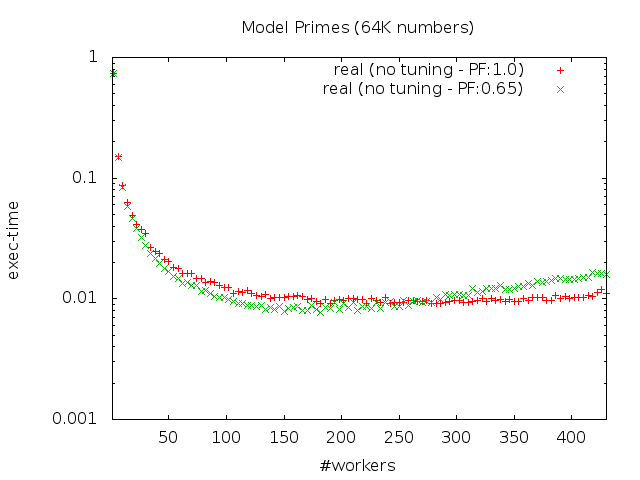
\includegraphics[width=0.55\paperwidth]{../BPG/images/MWfeatures-model.png}
	\caption{Real application execution time for partition factor values 1.0 and 0.65.}
	\label{fig:MWprimes-exhaustive}
\end{figure}

\begin {comment}

\paragraph{Best practice for choosing the initial number of workers}\label{para:mw-choose}\mbox{}\\

The results so far demonstrate that the analytical models implemented in the Master-Worker plugin produce quite accurate results. However, it can be statistically demonstrated that the partition factor estimated to balance the application for a certain number of workers is likely to be invalid if the number of workers changes significantly. This effect could be particularly adverse as the number of workers increases as load imbalances can reappear.

We will follow the case presented in the previous section to exemplify this issue and to show how to correct it. The plugin has estimated a partition factor of 0.65 to balance the application for 10 workers and it has subsequently estimated that the application can exploit 188 workers efficiently. This is a significant change from 178 workers {\color{red} Comment from ML: "178 workers? - where has this been mentioned before??" }   and, consequently, it is likely that the partition factor of 0.65 will not achieve good load balancing for this number of workers. This effect can be appreciated in Figure \ref{fig:MWprimes-exhaustive} because, even though the minimum execution time is obtained for 186 workers, the number of workers that are efficiently used should be approximately 150 workers. The best practice to correct this deviation is to execute PTF again, but using as the initial number of workers the results obtained in the first execution (206 in the example).  {\color{red} Comment from ML: "but using as the initial number of workers the results obtained in the first execution (206 in the example" - this is confusing - what is meant here?}

In this case, the first tuning step will produce the estimation shown in Table \ref{tab:mw-pf-estimation-206} for different values of the partition factor. This time, the plugin chooses 0.6 as the best partition factor. Next, the plugin estimates that the best number of workers in this case is 219 and generates the nine scenarios shown in Table \ref{tab:mw-plug-res-206} (along with the execution time of each scenario).

\begin{table}
    \centering
    \begin{tabular}{|c | c|}
    \hline
 {Partition Factor} &{Estimated Execution Time}\\\hline\hline
 0.10 & 0.01699\\
0.15 & 0.01677\\
0.20 & 0.01669\\
0.25 &  0.01662\\
0.30 & 0.01657\\
0.35 &  0.01653\\
0.40 &  0.01651\\
0.45 & 0.01649\\
0.50 & 0.01648\\
0.55 & 0.01645\\
0.60 & 0.01642\\
0.65 & 0.01644\\
0.70 & 0.01650\\
0.75 & 0.01671\\
0.80 & 0.01689\\
0.85 & 0.01709\\
0.90 & 0.01696\\
0.95 & 0.01762\\\hline
    \end{tabular}
    \caption{Estimation of the application execution time using 206 workers for different values of the partition factor.}
\label{tab:mw-pf-estimation-206}
\end{table}

Based on these results, the Master-Worker plugin advises the user to choose a partition factor of 0.54 and 240 workers. This advice is reliable as the means to reduce the imbalance when using more workers is to reduce the partition factor. Figure \ref{fig:MWprimes-exhaustive-206} shows the execution time of the application using a partition factor of 1.0, 0.65 and 0.54, respectively, in the range 4 to 430 workers. It can be seen that using a partition factor of 0.54 reduces the execution time of the application even more, and that the best time is obtained with 238 workers.

\begin{table}
    \centering
    \begin{tabular}{|c | c| c| c|}
    \hline
 {Scenario} &{Execution Time}& {Partition Factor} & {Number of Workers} \\\hline\hline
0  & 0.05506 & 0.54  & 198\\
1  & 0.05137 & 0.54  & 219\\
2  &  0.04966 & 0.54  & 240\\
3  & 0.05251 & 0.60  & 198\\
4  & 0.05553 & 0.60 & 219\\
5  &  0.05315 & 0.60 & 240\\
6  &  0.05410 & 0.66 & 198\\
7  & 0.05363 & 0.66 & 219\\
8  & 0.05200 & 0.66 & 240\\\hline
    \end{tabular}
    \caption{Results for the plugin generated scenarios.}
\label{tab:mw-plug-res-206}
\end{table}

Summarizing, if the tuning process with PTF advises a number of workers which is significantly larger than the one used to estimate the partition factor (the one indicated by the user in the execution command) then repeating the experiment using the advised number of workers will likely produce a better combination of the tuning parameters.

\begin{figure}[bt]
  \center
  \includegraphics[width=0.55\paperwidth]{../BPG/images/MWfeatures-model-206.png}
	\caption{Real application execution time for partition factor values 1.0, 0.65 and 0.54.}
	\label{fig:MWprimes-exhaustive-206}
\end{figure}
\end{comment}


\subsubsection{Uninstrumented applications supported for number of workers}\label{para:mw-unints}

The Master-Worker plugin cannot use analytical models for estimating the partition factor and number of workers if the application is not instrumented or it does not include a partition factor variable in its source code.  However, the plugin includes the possibility of tuning only the number of workers using an exhaustive search strategy. In this case, the user can just specify the range of workers and the step of the search. For example, the forest fire propagation application S2F2M \cite{Mostaccio05}  does not include a mechanism for load balancing (partition factor). In this case, we specify the range of 32 to 192 workers with step 4. The results obtained by PTF are shown in Table \ref{tab:mw-plug-res-s2f2m}, where it can be seen that the plugin advises the user to choose 176 workers (scenario 36).

\begin{table}
    \centering
    \begin{tabular}{|c | c| c|}
    \hline
 {Scenario} &{Execution Time}& {Number of Workers} \\\hline\hline
0	&	53.376	&	32	\\
1	&	47.975	&	36	\\
2	&	43.410	&	40	\\
3	&	39.664	&	44	\\
4	&	36.662	&	48	\\
5	&	34.372	&	52	\\
%6	&	32.206	&	56	\\
%7	&	30.237	&	60	\\
%8	&	28.815	&	64	\\
%9	&	27.479	&	68	\\
%10	&	26.202	&	72	\\
%11	&	25.220	&	76	\\
%12	&	24.361	&	80	\\
%13	&	23.516	&	84	\\
%14	&	22.545	&	88	\\
%15	&	21.873	&	92	\\
%16	&	21.132	&	96	\\
%17	&	20.664	&	100	\\
%18	&	19.933	&	104	\\
%19	&	19.581	&	108	\\
%20	&	19.119	&	112	\\
%21	&	19.453	&	116	\\
%22	&	18.357	&	120	\\
...	&	...		&	...	\\
%23	&	17.901	&	124	\\
%24	&	18.127	&	128	\\
%25	&	18.151	&	132	\\
%26	&	18.227	&	136	\\
27	&	19.196	&	140	\\
28	&	19.428	&	144	\\
29	&	17.815	&	148	\\
30	&	17.361	&	152	\\
31	&	18.008	&	156	\\
32	&	17.069	&	160	\\
33	&	17.520	&	164	\\
34	&	17.940	&	168	\\
35	&	17.374	&	172	\\
36	&	15.983	&	176	\\
37	&	17.337	&	180	\\
38	&	17.213	&	184	\\
39	&	16.546	&	188	\\
40	&	17.181	&	192	\\\hline
    \end{tabular}
    \caption{Results for the plugin generated scenarios.}
\label{tab:mw-plug-res-s2f2m}
\end{table}




